\documentclass[a4,danish]{article}

\usepackage{amssymb}
\usepackage{amsmath}
\usepackage{xcolor}
\usepackage{soul}
\usepackage{enumerate}

% Def, theorems, etc.
\usepackage{amsthm}
\newtheoremstyle{break}
	{\topsep}{\topsep}
	{\bfseries}{}
	{\newline}{}
\theoremstyle{break}
\newtheorem{theorem}[subsection]{Theorem}
\newtheorem{lemma}[subsection]{Lemma}
\newtheorem{proposition}[subsection]{Proposition}
\newtheorem{corollary}[subsection]{Corollary}
\theoremstyle{definition}
\newtheorem{definition}[subsection]{Definition}
\newtheoremstyle{Break}
	{\topsep}{\topsep}
	{}{}
	{\bfseries}{}
	{\newline}{}
\theoremstyle{Break}
\newtheorem{example}[subsection]{Example}
\newtheorem{remark}[subsection]{Remark}
\newtheorem{note}[subsection]{Note}
\setcounter{secnumdepth}{0}
\usepackage{xpatch}
\xpatchcmd{\proof}{\ignorespaces}{\mbox{}\\\ignorespaces}{}{}


\newcommand{\Z}{\mathbb{Z}}
\newcommand{\Q}{\mathbb{Q}}
\newcommand{\R}{\mathbb{R}}
\newcommand{\N}{\mathbb{N}}
\newcommand{\C}{\mathbb{C}}
\newcommand{\I}{\text{Imm}}
\renewcommand{\S}{\mathbb{S}}
\renewcommand{\P}{\text{P}}
\newcommand{\blank}{\makebox[1ex]{\textbf{$\cdot$}}}
\renewcommand{\phi}{\varphi}
\renewcommand{\epsilon}{\varepsilon}

\newcommand*\diff{\mathop{}\!\mathrm{d}}

\setlength{\parskip}{1em}
\setlength{\parindent}{0em}

% Figures -- use this instead of full file path because of git.
\usepackage{graphicx}
\graphicspath{{../figures/}}

\title{The tangent space of closed curves in $\R^2$}
\author{Mads and Anders}
\date{\today}

\begin{document}
% \maketitle

\section*{The manifold of curves}
\label{sec:manifold-curves}

By \hl{(some reference)} ...

\section*{The tangent space of curves}
\label{sec:tangent-space-closed}



\paragraph{Constructing the space of closed curves.}
Intuitively, we want to consider the space of all (smooth) closed
curves in $\R^2$. This can be seen as the space of all submanifolds in
$\R^2$ which are diffeomorphic to the unit circle $\S^1$. If we let
$\text{Imm}(\S^1,\R^2)$ denote the space of all \textit{immersion}
from the inut circle into the plane, we can define the space we
want to consider as
\begin{equation}
  \label{eq:curves}
  B :=
  \left\{
    q(\S^1) \mid q \in \text{Imm}(\S^1,\R^2)
  \right\}.
\end{equation}
Here we simply think of $q(\S^1) \subset \R^2$ as a subspace and forget
about the actual map $q$. (Keeping this mapping in mind we could
define the space in another way; but this is not so important right
now.)

\paragraph{The tangent space of B.}
For ordinary finite dimensional manifolds $B$, Lee defines the tangent
space at a point $p \in B$ through the notation of
\textit{derivations}; this is a rather abstract construction, but is
nice to work with. Using this, one can define the notion of a
tanget vector to a path in $B$ passing through the point $p$. Then,
one can define an equivalence relation on the space of such paths and
obtain an equivalent definition of the tanget space, which is more
intuitive. One can also work the other way around and start by
defining the notion of tanget vector to paths in $B$ (as is done on
Wiki). We briefly do that here:

For a neighbourhood $U \subset B$ containing $p$ we have a smooth coordinate
chart $\phi\colon U \rightarrow \R^n$. For a path $\gamma \colon
[-\epsilon,\epsilon] \rightarrow B$ with $\phi(0) = p$, it makes perfect sense to consider
differentiability of the map $\phi \circ \gamma \colon
[0,1]\rightarrow \R^n$. Now, the relation
\begin{equation*}
  \gamma_1 \sim \gamma_2 \iff
  (\phi \circ \gamma_1)'(0) = (\phi \circ \gamma_2)'(0),
\end{equation*}
defines an equivalence relation on the collection of all such paths
$\gamma$. An equivalence class of such paths, denoted by $[\gamma'_p]$ (or simply
$\gamma'_p$), is called a \textit{tangent vector}
at the point $p$. The collection of all tanget vectors make up the
tanget space $T_pB$ at $p$.

Returning to $B$ being as defined in (\ref{eq:curves}), we now
want to determine what the tangent spaces look like at a point $q \in B$ by
following the construction above (taking for
granted that $B$ actually is a (Fr\'echet) manifold, and
that the following definitions/constructions make sense). Firstly, a
path in $B$ is now a map $\gamma\colon [-\epsilon,\epsilon] \rightarrow B$ such that
$\gamma(t)$ is a curve $q_t \in B$ for all $t \in
[-\epsilon,\epsilon]$, with $\gamma(0) =q$. For each of the $q_t$ we
can think of them as parametrized by $x \mapsto q_t(x)$, $x \in
\S^1$. Then, if the curve $\gamma$ is such that for each fixed
$x \in \S^1 $ the map $t \mapsto q_{t}(x) \in \R^2$ is differentiable,
we can define $\gamma'_q$ as the mapping
\begin{equation*}
  \gamma'_q := x \mapsto \frac{\partial }{\partial t} \bigg\vert_{t=0}q_t(x).
\end{equation*}
Thus each $\gamma'_q$ is a mapping from the unit circle into $\R^2$,
which mean that we can think of a tangent vector to a curve $q \in B$
as a vector field on $\S^1$ (though of as $\subset \R^2$).


\paragraph{Question / considerations / imprecisions.}
Above we made an intuitively reasonable construction, but ignored some
of technicalities, which we list here.
\begin{itemize}
\item Equivalence classes: We should define the tangent vectors as
  equivalence classes of path in $B$; this should all determine a
  unique vector field.
\item The manifold structure of $B$: We simply used the intuitive idea
  to differentiate in ``time'' for each fixed point on a curve,
  $q_t(x)$. However, as we have not specified the chart for the
  manifold $B$, it is not obvious that this construction corresponds
  to the one made in the finite dimensional case. Technically we
  would need a chart $\phi \colon U \rightarrow F$, with $F$ some
  Fr\'echet space and then show some sort of Fr\'echet-differentiability of the
  composite function $\phi \circ \gamma$.
\item We mentioned that in the finite dimensional case the two
  definitions (through derivates and tangents to curves, respectively)
  are equivalent. It is not obvious that this also hold in the
  infinite dimensional case.
\item At the beginning we eliminated the knowledge of the
  parametrization of a curve $q \in B$ to make the definition of $B$
  simpler. However, we actually use a parametrization later, and thus
  we should make sure that reparametrizations does not matter for the
  construction of the tangent space. (It does not, as it would just
  move the vector field around $\S^1$ according to the
  reparametrization.)
\item Are there any smoothness assumptions (or something) about vector
  field we need to validate? For example, just the fact that the map
  $t \mapsto q_t(x)$ behaves nice does of course \textit{not} imply
  that also the derived vector field $\gamma'_q$ behaves nicely in
  $x$ -- which is what we would need to get a smooth vector field
  (?).
\item Is it correctly formulated that we need to think of $\S^1
  \subset \R^2$ to make sense of a vector field on the circle?
\end{itemize}


% \section*{Test section}
% \label{sec:test-section}

% \begin{center}
%   \begin{tikzpicture}
%     \begin{axis}[axis lines=none, axis equal,
%       width=0.9\textwidth,
%       xmin=-3,xmax=10,
%       ymin=-3,ymax=3,
%       % grid=both,
%       ]
%       \addplot [domain=0:360,samples=100]({2*cos(x)},{2*sin(x)});
%       \addplot[domain=0:360,samples=200]({7 +
%         (1-cos(x*2)/2)*1.8*sin(x)},{(1-sin(x*4)/2)*1.8*cos(x)});
%       \node[anchor=west] (source) at (axis cs:1.0,2.5){}; \node
%       (destination) at (axis cs:5.5,2.5){}; \draw[->](source) to
%       [out=40,in=140] (destination);
%     \end{axis}
%   \end{tikzpicture}
% \end{center}

% \begin{center}
%   \begin{tikzpicture}
%     \begin{axis}[axis lines=none, axis equal,
%       width=1\textwidth,
%       xmin=4,xmax=10,
%       ymin=-4,ymax=4,
%       ]
%       \addplot[domain=0:360,samples=200]({7 +
%         (1-cos(x*2)/2)*1.8*sin(x)},{(1-sin(x*4)/2)*1.8*cos(x)});

%       \addplot[domain=0:360,samples=200]({7 +
%         (1-0*cos(x*2)/2)*1.8*sin(x)},{1.2*(1-sin(x*4)/2)*1.8*cos(x)});

%       \foreach \t in {1,...,4}
%       \addplot[gray, domain=0:360,samples=200]
%       ({7 + (1-(1-\t /5)*cos(x*2)/2)*1.8*sin(x)},
%       {(1 + \t /25)*(1-sin(x*4)/2)*1.8*cos(x)});

%       \foreach \q in {1,...,72}
%       \addplot[->, red, domain=0:2.5,samples=5]
%       ({7 + (1-(1-x /5)*cos(\q *5*2)/2)*1.8*sin(\q *5)},
%       {(1 + x /25)*(1-sin(\q *5*4)/2)*1.8*cos(\q *5)});
%     \end{axis}
%   \end{tikzpicture}
% \end{center}


% \begin{center}
%   \begin{tikzpicture}
%     \begin{axis}[axis lines=none, axis equal,
%       width=1\textwidth,
%       xmin=4,xmax=10,
%       ymin=-4,ymax=4,
%       ]
%       \addplot[domain=0:360,samples=200]({7 +1 +
%         2*sin(x)},{2*cos(x)});

%       \foreach \q in {1,...,72}
%       \addplot[->, green, domain=0:2.5,samples=5]
%       ({7 + (1-(1-x /5)*sin(\q *5)*2},
%       {(1 + x /25)*2*cos(\q *5)});
%     \end{axis}
%   \end{tikzpicture}
% \end{center}

\section*{Defining a metric on the tangent space of curves 1}
\label{sec:defin-metr-tang}

\hl{This is the sort of argument they (Mumford and Michor) give in the
  beginning of section 3.2. Not sure how to exactly finish this.}

Consider the following metric on $\I$.

\begin{definition}[The L2 metric on $\I$]
  The \textit{L2 metric} $G^2_c$ at the point $c \in \I$ is defined as
  \begin{equation*}
    G^2_c(h,k) := \int_{\S^{1}} \left\langle{h(\theta)
    , k(\theta)}\right\rangle |c_{\theta}| \diff \theta,
  \end{equation*}
  $h,k \in T_cB = C^{\infty}(\S^1,\R^2)$.
\end{definition}

Adding the parametrization derivative $c_{\theta}$ makes this
invariant under \hl{(orientation preserving?)}
reparametrizations. Because of that, this metric also induces a metric
on the quotient space $B$, which we can identify as follows. Consider
first the tangent space at $c$ to the \textit{orbit} of the diffeomorphism
group
\begin{equation*}
  T_c(c \circ \text{Diff}(\S^{1})), \quad c \circ
  \text{Diff}(\S^{1}) := 
  \left\{
    c \circ \phi \mid \phi \in \text{Diff}(\S^{1})
  \right\} .
\end{equation*}
A path in the orbit $c \circ \text{Diff}(\S^{1})$ reduces to
\begin{equation*}
  t \mapsto 
  \left(
    \theta \mapsto (c \circ \phi_t) (\theta)
\right).
\end{equation*}
Differentiating this with respect to $t$ shows that we can identify
\begin{equation}
  \label{eq:tang-orbit}
  T_c(c \circ \text{Diff}(\S^{1})) = 
  \left\{
    g c_{\theta} \mid g \in C^{\infty}(\S^1, \R)
  \right\}.
\end{equation}
The \textit{normal space} $\mathcal{N}_c \subset T_c(\I)$ consists of
tangent vectors that are orthogonal to $T_c(c \circ
\text{Diff}(\S^{1}))$ with respect to $G_c^2$. As the projection
\begin{equation*}
  \pi \colon \I \rightarrow B = \I/\text{Diff}(\S^{1})
\end{equation*}
sends the whole orbit to a single point \hl{it follows} that tangents
vectors to the projected element $\pi(c) \in B$ can essentially
be identified with elements of the normal space $\mathcal{N}_c$.
From \eqref{eq:tang-orbit} we see that
\begin{equation*}
  \mathcal{N}_c =
  \left\{
    g i c_{\theta} \mid g \in C^{\infty}(\S^1, \R)
  \right\},
\end{equation*}
with $i c_{\theta} = |c_{\theta}| n_c$, $n_c$ being the unit normal
vector field along $c$. Finally, for a given $h \in T_c(\I)$
we can explicitly find the decomposition of $h$ into the two orthogonal
subspaces of the tangent space by projecting $h$ onto $c_{\theta}$ and
$ic_{\theta}$, which gives
\begin{equation*}
  \begin{aligned}
    h &  = p_{c_{\theta}}(h) + p_{ic_{\theta}}(h)
    \in T_c(c \circ \text{Diff}(\S^{1})) \oplus \mathcal{N}_c
    ,\\
    p_{c_{\theta}}(h) & = 
    \frac{\langle h, c_{\theta}\rangle}{|c_{\theta}|^2} c_{\theta}
    \in T_c(c \circ \text{Diff}(\S^{1})), \\
    p_{ic_{\theta}}(h) & = 
    \frac{\langle h, ic_{\theta}\rangle}{|c_{\theta}|^2} ic_{\theta}
    \in \mathcal{N}_c,
  \end{aligned}
\end{equation*}
with $p_{v}(u)$ denoting the standard orthogonal projection in $\R^2$.

This allows us to calculate a formula for
the induced metric on $B$. In particular, it allows us to explicitly calculate
the length of a projected path $t \mapsto \pi(q(t,\blank)) \in B $
where $t \mapsto q(t,\blank) \in \I$ is a path in $\I$.
In this setting, at each time point $t$
the tangent vector is $q_t$ so \hl{by the above arguments} we get that
the induced metric is
\begin{equation*}
  \begin{aligned}
    L^2(\pi(q))& = \int_{0}^{1}
    G^2_{q(t,\blank)}(p_{iq_{\theta}}(q_t),p_{iq_{\theta}}(q_t)) \diff t \\
    & = \int_{0}^{1}
    \int_{\S^1} 
    \left\langle
      \frac{\langle h, iq_{\theta}\rangle}{|q_{\theta}|^2} iq_{\theta},
      \frac{\langle h, iq_{\theta}\rangle}{|q_{\theta}|^2} iq_{\theta}
  \right\rangle | q_{\theta}|\diff \theta \diff t.
  \end{aligned}
\end{equation*}


\section*{Defining a metric on the tangent space of curves 2}
\label{sec:defin-metr-tang-2}



\begin{definition}[The L2 metric on $\I$]
  The \textit{L2 metric} $G^2_c$ at the point $c \in \I$ is defined as
  \begin{equation*}
    G^2_c(h,k) := \int_{\S^{1}} \left\langle{h(\theta)
    , k(\theta)}\right\rangle |c_{\theta}| \diff \theta,
  \end{equation*}
  $h,k \in T_cB = C^{\infty}(\S^1,\R^2)$.
\end{definition}

Because this metric is invariant under reparametrizations it also induces a metric
on the quotient space $B = \I/\text{Diff}(\S^1)$ and thus 
determines a length measure on the paths in $B$
\hl{[define this]}. We want to find an expression for this, using
parametrized representatives from $\I$. For a parametrized curve $c
\in \I$ we write $C = \text{Im}(c) =: \pi(c) \in B$ for the projection
onto the quotient space. For any path $t \mapsto q(t, \blank) \in
\I$ running through the space of parametrized curves, this induces
a path in $B$ by simply projecting the path down to $t \mapsto \pi(q(t,
\blank))$. 

In ... it is shown that ... We here give some intuitive, geometric
arguments for why this should be true.

We know that a tangent vector $h$ to a curve $c \in \I$ can be visualized
as a vector field on the circle. By definition, this vector field is
derived from a path $t \mapsto q(t,\blank)$ in $\I$ as $h =q_t(0,\blank)$.
At each of the
timepoints, $t$, we get a particular parametrized curve $\theta
\mapsto q(t,\theta)$. We cannot directly use such a path to define
tangent vectors of the \textit{quotient space} $B$ because this path is
sensitive to reparametrizations: Consider a time-dependent
reparametrization $\phi(t,\theta)$, or, equivalently, a path $t \mapsto \phi(t,
\blank)$ in $\text{Diff}(\S^1)$; then the two paths $t \mapsto
\pi(q(t, \blank))$ and $t \mapsto \pi(q(t, \phi(t, \blank)))$ are
identical in $B$ but give rise to two different vector fields.

To make better sense of the tangents vectors of the quotient space, we
use the following result.

\begin{proposition}
  \label{prop:horizontal-path}
  For every path $t \mapsto q(t, \blank)$ in $\mathrm{Imm}$ there exists a
  time-dependent reparametrization $t \mapsto \phi(t, \blank) \in
  \mathrm{Diff}(\S^{1})$ such that the path
  \begin{equation*}
    t \mapsto r(t, \theta):=q(t, \phi(t,\theta))
  \end{equation*}
  fulfills
  $\langle e_t, e_{\theta}\rangle=0$ for all $(t,\theta) \in [0,1]\times \S^1$. For
  the reparametrization $\phi$ it holds that $\phi(0, \theta)=\theta$ and that
  \begin{equation}
    \label{eq:canon-repar}
    \phi_t = a \circ \phi, \quad a := -\frac{\langle q_t,
      q_{\theta}\rangle}{|q_{\theta}|^2}.
  \end{equation}
\end{proposition}

\begin{proof}
  \hl{todo or ref.}
\end{proof}

\begin{remark}
  Note that for every vector field $h \in T_c(\I)$, determined from the path $q$, we can make a pointwise decomposition of $h$ onto $q_{\theta}(0, \blank)$ and $iq_{\theta}(0, \blank)$ by using the pointwise orthogonal projection. Explicitly we have that
  \begin{equation*}
    h = q_t = p_{q_{\theta}}(q_{t}) + p_{iq_{\theta}}(q_{t}), 
  \end{equation*}
  where $p$ is taken to be the standard \textit{pointwise} $\R^2$ orthogonal projection, which is given as
  \begin{equation*}
    p_v(u) = \frac{\langle v, u \rangle}{|v|^2} v, \quad u, v \in \R^2.
  \end{equation*}
  More correctly we should thus write
  \begin{equation*}
    h(\theta) = q_t(0,\theta) = p_{q_{\theta}(0,\theta)}(q_{t}(0,\theta)) +
    p_{iq_{\theta}(0,\theta)}(q_{t}(0,\theta)).
  \end{equation*}
  From this we see that the time derivative of the reparametrization in the previous Proposition is the coefficient function for the projection onto the parameter derivative of the original path $q$; this becomes relevant in a moment. 
\end{remark}

We can use this result to define tangent vectors to elements of $B$ in
a consistent way:

\begin{definition}
  We define tangents vectors to be 
\end{definition}

For some path $q$ in $\I$, reparametrize this according to Proposition~\ref{prop:horizontal-path}; then take derivative as in the parametrized case of this new path. This leads us to the following result.

\begin{proposition}
  The tangent space to an element $C = \pi(c) \in B$ consists of orthonormal vector fields on the circle, i.e.,
  \begin{equation*}
    T_C(B) = 
    \left\{
      b i c_{\theta} \mid b \in C^{\infty}(\S^1,\R)
    \right\}
    = C^{\infty}(\S^1,\R).
  \end{equation*}
  For a path $t \mapsto q(t,\blank) \in \I$ such that 
\end{proposition}

\begin{proof}
  We have justified why this should be the case in the previous discussion, by defining a consistent way to construct the tangent space. 
\end{proof}

\section*{Test section 2}
\label{sec:test-section-2}

\begin{figure}
  \centerline{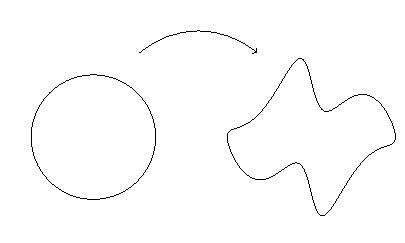
\includegraphics[width=0.7\linewidth]{circle_mapping.pdf}}
  % \caption[]{}
\end{figure}

\begin{figure}
  \centerline{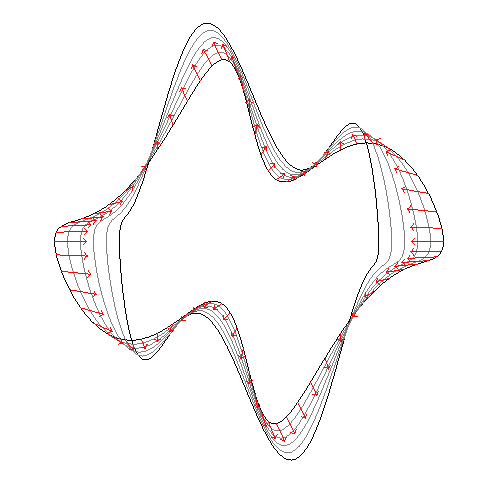
\includegraphics[width=0.7\linewidth]{path.pdf}}
  % \caption[]{}
\end{figure}

\begin{figure}
  \centerline{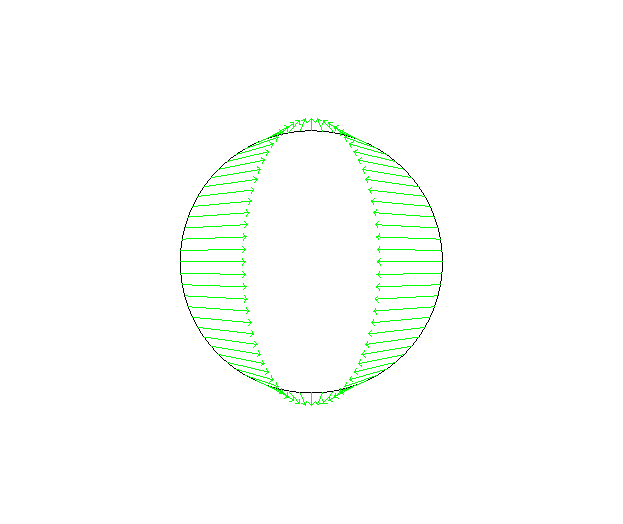
\includegraphics[width=0.7\linewidth]{circle_vectorfield.pdf}}
  % \caption[]{}
\end{figure}



\end{document}





